% !TeX root = ./main.tex

\section{Teorema da Aproximação Universal}

Nesta seção apresentaremos o principal resultado estudado: o teorema da aproximação universal, como formulado em \cite{cybenko89}.
Ele trata, assim como o teorema da aproximação de Weierstrass, da tarefa de aproximar funções reais contínuas.
Porém, agora nossas funções alvo são definidas em \( \I^{ n } \), o hipercubo unitário \( n \)-dimensional, e a classe de funções que temos à nossa disposição para obter essas aproximações é a das funções definidas como somas da forma
\begin{equation}
    x \mapsto \sum_{ j=1 }^{ N } \alpha_{ j } \sigma(y_{ j }^{ T }x + \theta_{ j })
    \label{eq: neural_func}
,\end{equation}
onde \( \alpha_{ j }, \theta_{ j } \in \R \), \( y_{ j } \in \R^{ n } \) para todo \( 1 \leq j \leq N \) são parâmetros e a função pré-fixada \( \sigma : \R \to \R \) é uma \emph{sigmoide}, ou seja, é tal que \[
    \sigma(x) \to
    \begin{cases}
        1, \text{ se } x \to +\infty \\
        0, \text{ se } x \to -\infty
    \end{cases}
.\]
Como pode-se ver, a função \( \sigma \) é a componente \emph{não-linear} da aproximação.
Apesar de agora essa parecer uma escolha muito peculiar, funções do tipo apresentado em (\ref{eq: neural_func}) são muito relevantes em várias aplicações, como a próxima subseção deixará mais claro.

Como o leitor pode lembrar, quando abordamos o \( 13^{ \circ } \) problema de Hilbert enunciamos o caso geral e provamos um caso particular do teorema da superposição de Kolmogorov, segundo o qual podemos representar de forma \emph{exata} funções contínuas de \( \I^{ n } \) em \( \R \) utilizando a superposição e composição de funções contínuas de \( \I \) em \( \R \), de uma maneira parecida como a apresentada em (\ref{eq: neural_func}).
Entretanto, como comentado em \cite{cybenko89}, a diferença crucial entre esses dois resultados é que no teorema de Kolmogorov nos é permitido usar uma classe muito maior de não-linearidades, as quais variam de acordo com a função a ser aproximada.

\subsection{Redes Neurais Artificiais}

Como descrito em \cite{lipmann}, as redes neurais artificiais são algoritmos de computação que surgiram como uma tentativa de espelhar o funcionamento de redes neurais orgânicas, como o cérebro humano.
Em essência, seu objetivo é ``atingir bom desempenho por meio da densa interconexão de elementos computacionais simples.''

Na prática, existem várias formas de atingir esse objetivo.
No tipo de rede ao qual daremos enfoque, o processo de computação é realizado por um conjuntos de nós, organizados em camadas ordenadas, em que a camada inicial é composta por \( n \) nós de \verb|input| e a camada final, por \( m \) nós de \verb|output|.
Entre eles a rede pode possuir camadas intermediárias de tamanho variado.
Dados \( n \) valores reais para os nós de \verb|input|, a rede produz, nos nós de \verb|output|, \( m \) valores, também reais.
Logo, ela pode ser considerada uma função de \( \R^{ n } \) em \( \R^{ m } \).

A partir da segunda camada, cada nó está conectado a todos os nós da camada anterior por meio de uma aresta, a qual possui um peso.
Esse nó computa uma combinação linear, utilizando como coeficientes os pesos das arestas, dos valores armazenados pelos nós da camada anterior, soma um fator de correção ao valor obtido e passa o resultado por uma função não-linear, obtendo assim um valor próprio.
O caso em que \( m = 1 \) e há apenas uma camada intermediária, ao qual nos atentaremos, está representado na figura \ref{fig: neural_net}, utilizando uma sigmoide como não-linearidade.

\begin{figure}[htb]
    \begin{center}
        % !TeX root = ../main.tex

\tikzset{%
  every neuron/.style={
    circle,
    draw,
    minimum size=1cm
  },
  neuron missing/.style={
    draw=none, 
    scale=3,
    text height=0.3cm,
    execute at begin node=\color{black}$\vdots$
  },
}

\vspace{.6cm}

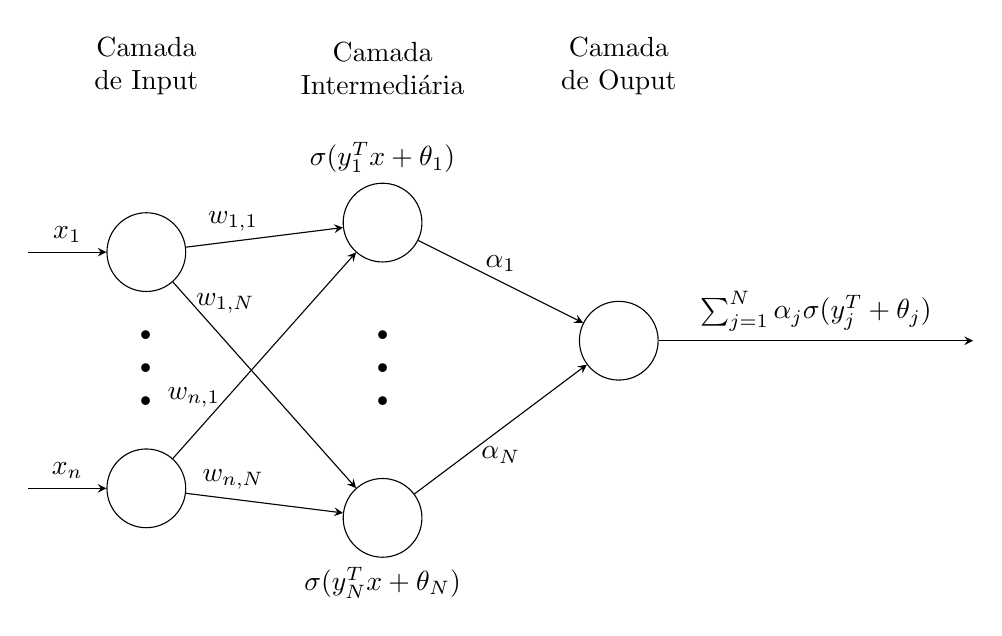
\begin{tikzpicture}[x=1.5cm, y=1.5cm, yshift=-1, >=stealth]

\foreach \m/\l [count=\y] in {1,missing,2}
  \node [every neuron/.try, neuron \m/.try] (input-\m) at (0,1.75-\y) {};

\foreach \m [count=\y] in {1,missing,2}
  \node [every neuron/.try, neuron \m/.try ] (hidden-\m) at (2,2.25-\y*1.25) {};

\foreach \m [count=\y] in {1}
  \node [every neuron/.try, neuron \m/.try ] (output-\m) at (4,1-\y) {};

\foreach \l [count=\i] in {1,n}
  \draw [<-] (input-\i) -- ++(-1,0)
    node [above, midway] {$x_\l$};

%% \foreach \l [count=\i] in {1,n}
%%   \node [above] at (hidden-\i.north) {$H_\l$};
\node [above] at (hidden-1.north) {\( \sigma (y_{ 1 }^{ T }x + \theta_{ 1 }) \)};
\node [below] at (hidden-2.south) {\( \sigma (y_{ N }^{ T }x + \theta_{ N }) \)};

\foreach \l [count=\i] in {1}
  \draw [->] (output-\i) -- ++(3,0)
    node [above, midway] {\( \sum_{ j=1 }^{ N } \alpha_{ j } \sigma (y_{ j }^{ T } + \theta_{ j }) \)};

%% \foreach \i in {1,...,2}
%%   \foreach \j in {1,...,2}
%%     \draw [->] (input-\i) -- (hidden-\j)
%%         node [above,pos=.2] {\( y_{ 1 }^{ (1) } \)};
\draw [->] (input-1) -- (hidden-1)
    node [above, pos=.3] {\( w_{ 1,1 } \)};
\draw [->] (input-2) -- (hidden-1)
    node [above, pos=.2, xshift=-2mm] {\( w_{ n,1 } \)};
\draw [->] (input-1) -- (hidden-2)
    node [above, pos=.2,xshift=2mm] {\( w_{ 1,N } \)};
\draw [->] (input-2) -- (hidden-2)
    node [above, pos=.3] {\( w_{ n,N } \)};

%% \foreach \i in {1,...,2}
%%   \foreach \j in {1}
%%     \draw [->] (hidden-\i) -- (output-\j);
\draw [->] (hidden-1) -- (output-1)
    node [above, midway] {\( \alpha_{ 1 } \)};
\draw [->] (hidden-2) -- (output-1)
    node [below, midway, yshift=-1mm] {\( \alpha_{ N } \)};

\foreach \l [count=\x from 0] in {de Input, Intermediária, de Ouput}
  \node [align=center, above] at (\x*2,2) {Camada \\ \l};

\end{tikzpicture}
    \end{center}
    \caption{Rede neural com apenas uma camada intermediária.
    Aqui temos \( x =
    \begin{bmatrix}
        x_{ 1 } & \cdots & x_{ n }
    \end{bmatrix}^{ T } \) e \( y_{ j }^{ T }x =
    \begin{bmatrix}
        w_{ 1,j } & \cdots & w_{ n,j }
    \end{bmatrix} \), o vetor dos pesos de cada nó intermediário.
    Na última camada ocorre apenas uma combinação linear.
    Repare que o output da rede é exatamente a expressão em (\ref{eq: neural_func}).}
    \label{fig: neural_net}
\end{figure}

Ou seja, o nosso objetivo nessa seção é estudar se podemos aproximar funções reais contínuas em \( \I^{ n } \) utilizando redes neurais com uma camada intermediária.
Essa é uma pergunta de extrema relevância, tanto teórica como prática pois, como apontado em \cite{lipmann}, redes neurais artificiais possuem diversas aplicações em campos voltados ao desenvolvimento de classificadores robustos, como a teoria de reconhecimento de fala e de imagens.
Saber que é possível realizar aproximações arbitrariamente boas utilizando redes neurais artificiais dá mais segurança e incentivo à pesquisa nessas áreas.

\subsection{O Teorema}

Denotaremos o espaço das funções reais contínuas em \( \I^{ n } \) por \( C(\I^{ n }) \) e o espaço das medidas de Borel finitas, com sinal e regulares em \( \I^{ n } \) por \( M(\I^{ n }) \).
Queremos entender sob quais condições as somas da forma \[
    G(x) = \sum_{ j=1 }^{ N } \alpha_{ j } \sigma(y_{ j }^{ T }x + \theta_{ j })
\]
são densas em \( C(\I^{ n }) \) com respeito à norma do supremo.
Faremos isso primeiro para uma classe mais geral de funções \( \sigma \) e depois mostraremos que as sigmoides pertencem a essa classe.

\begin{defn}
    Dizemos que \( \sigma \) é \emph{discriminatória} se, para uma medida \( \mu \in M(I^{ n }) \), termos \[
        \int_{ \I^{ n } } \sigma(y^{ T }x + \theta)  \ \mathrm{d}\mu = 0
    \]
    para todos \( y \in \R^{ n } \) e \( \theta \in \R \) implica em \( \mu = 0 \).
\end{defn}

\begin{teo}[Teorema da aproximação universal]
    Seja \( \sigma \) uma função contínua discriminatória qualquer.
    Então as somas finitas da forma \[
        G(x) = \sum_{ j=1 }^{ N } \alpha_{ j } \sigma(y_{ j }^{ T }x + \theta_{ j })
    \]
    são densas em \( C(\I^{ n }) \).
    Em outras palavras, dada qualquer \( f \in C(\I^{ n }) \) e \( \varepsilon > 0 \), existe uma soma, \( G(x) \), da forma acima, tal que \[
        \norm{ G - f }_{ \infty } < \varepsilon
    .\]
\end{teo}


